\documentclass{beamer}
\usepackage{../../shared/styles/custom}
% =============================================================================
% ML TEACHING MATHEMATICAL NOTATION CONVENTIONS
% =============================================================================
% Based on standard ML textbooks: Murphy's "Machine Learning: A Probabilistic Perspective",
% Bishop's "Pattern Recognition and Machine Learning", and "Mathematics for Machine Learning"

% =============================================================================
% CORE NOTATION STANDARDS
% =============================================================================

% SCALARS: Regular italics (lowercase for variables, uppercase for constants)
% Examples: x, y, n, d, k, \theta, \alpha, \lambda, \sigma

% VECTORS: Bold lowercase letters
% Examples: \mathbf{x}, \mathbf{w}, \mathbf{\mu}, \mathbf{\theta}

% MATRICES: Bold uppercase letters
% Examples: \mathbf{X}, \mathbf{W}, \mathbf{\Sigma}, \mathbf{\Lambda}

% SETS: Calligraphic uppercase
% Examples: \mathcal{D}, \mathcal{X}, \mathcal{Y}

% SPACES: Blackboard bold
% Examples: \mathbb{R}, \mathbb{Z}, \mathbb{N}

% =============================================================================
% VECTOR NOTATION (bold lowercase)
% =============================================================================

\newcommand{\vx}{\mathbf{x}}        % Input vector
\newcommand{\vy}{\mathbf{y}}        % Output vector
\newcommand{\vw}{\mathbf{w}}        % Weight vector
\newcommand{\vb}{\mathbf{b}}        % Bias vector
\newcommand{\vh}{\mathbf{h}}        % Hidden vector
\newcommand{\vz}{\mathbf{z}}        % Latent vector
\newcommand{\vf}{\mathbf{f}}        % Function vector
\newcommand{\vg}{\mathbf{g}}        % Gradient vector
\newcommand{\vu}{\mathbf{u}}        % Generic vector u
\newcommand{\vv}{\mathbf{v}}        % Generic vector v
\newcommand{\vzero}{\mathbf{0}}     % Zero vector
\newcommand{\vone}{\mathbf{1}}      % Ones vector

% Greek vectors (bold)
\newcommand{\vmu}{\boldsymbol{\mu}}     % Mean vector
\newcommand{\vtheta}{\boldsymbol{\theta}} % Parameter vector
\newcommand{\vlambda}{\boldsymbol{\lambda}} % Lambda vector
\newcommand{\valpha}{\boldsymbol{\alpha}}   % Alpha vector
\newcommand{\vbeta}{\boldsymbol{\beta}}     % Beta vector
\newcommand{\vxi}{\boldsymbol{\xi}}         % Xi vector
\newcommand{\vepsilon}{\boldsymbol{\epsilon}} % Epsilon vector

% =============================================================================
% MATRIX NOTATION (bold uppercase)
% =============================================================================

\newcommand{\mX}{\mathbf{X}}        % Data matrix
\newcommand{\mY}{\mathbf{Y}}        % Target matrix
\newcommand{\mW}{\mathbf{W}}        % Weight matrix
\newcommand{\mA}{\mathbf{A}}        % Generic matrix A
\newcommand{\mB}{\mathbf{B}}        % Generic matrix B
\newcommand{\mC}{\mathbf{C}}        % Generic matrix C
\newcommand{\mH}{\mathbf{H}}        % Hidden layer matrix / Hessian
\newcommand{\mI}{\mathbf{I}}        % Identity matrix
\newcommand{\mJ}{\mathbf{J}}        % Jacobian matrix
\newcommand{\mK}{\mathbf{K}}        % Kernel matrix
\newcommand{\mL}{\mathbf{L}}        % Loss matrix / Cholesky factor
\newcommand{\mP}{\mathbf{P}}        % Projection matrix
\newcommand{\mQ}{\mathbf{Q}}        % Orthogonal matrix
\newcommand{\mR}{\mathbf{R}}        % Rotation matrix
\newcommand{\mS}{\mathbf{S}}        % Scatter matrix
\newcommand{\mU}{\mathbf{U}}        % Left singular vectors
\newcommand{\mV}{\mathbf{V}}        % Right singular vectors

% Greek matrices (bold)
\newcommand{\mSigma}{\boldsymbol{\Sigma}}   % Covariance matrix
\newcommand{\mLambda}{\boldsymbol{\Lambda}} % Diagonal eigenvalue matrix
\newcommand{\mPhi}{\boldsymbol{\Phi}}       % Feature matrix
\newcommand{\mPsi}{\boldsymbol{\Psi}}       % Basis matrix
\newcommand{\mTheta}{\boldsymbol{\Theta}}   % Parameter matrix

% =============================================================================
% SETS AND SPACES (following Bishop/Murphy conventions)
% =============================================================================

\newcommand{\cD}{\mathcal{D}}       % Dataset
\newcommand{\cH}{\mathcal{H}}       % Hypothesis space
\newcommand{\cX}{\mathcal{X}}       % Input space
\newcommand{\cY}{\mathcal{Y}}       % Output space
\newcommand{\cF}{\mathcal{F}}       % Function space
\newcommand{\cG}{\mathcal{G}}       % Gaussian process
\newcommand{\cL}{\mathcal{L}}       % Lagrangian / Loss
\newcommand{\cN}{\mathcal{N}}       % Normal distribution
\newcommand{\cU}{\mathcal{U}}       % Uniform distribution
\newcommand{\cB}{\mathcal{B}}       % Bernoulli distribution
\newcommand{\cP}{\mathcal{P}}       % Probability distribution

% Number systems
\newcommand{\Real}{\mathbb{R}}      % Real numbers
\newcommand{\Nat}{\mathbb{N}}       % Natural numbers
\newcommand{\Int}{\mathbb{Z}}       % Integers
\newcommand{\Complex}{\mathbb{C}}   % Complex numbers

% =============================================================================
% OPERATORS AND FUNCTIONS (following standard conventions)
% =============================================================================

% Prediction notation (commonly used in ML)
\newcommand{\yhat}{\hat{\vy}}        % Predicted output vector (bold)
\newcommand{\yhati}{\hat{y}_i}       % Predicted output for sample i (scalar)

% Common ML functions (with conflict resolution)
\providecommand{\sigmoid}{}
\renewcommand{\sigmoid}{\operatorname{sigmoid}}
\providecommand{\softmax}{}
\renewcommand{\softmax}{\operatorname{softmax}}
\providecommand{\ReLU}{}
\renewcommand{\ReLU}{\operatorname{ReLU}}
\providecommand{\sign}{}
\renewcommand{\sign}{\operatorname{sign}}
\DeclareMathOperator{\Gain}{Gain}    % Information gain
\DeclareMathOperator{\Entropy}{Entropy}
% KL divergence (check for conflicts)
\providecommand{\KL}{}
\renewcommand{\KL}{\operatorname{KL}}
\DeclareMathOperator{\MSE}{MSE}      % Mean squared error
\DeclareMathOperator{\MAE}{MAE}      % Mean absolute error
\DeclareMathOperator{\RMSE}{RMSE}    % Root mean squared error

% Classification metrics (upright text)
\newcommand{\TP}{\text{TP}}          % True positives
\newcommand{\TN}{\text{TN}}          % True negatives  
\newcommand{\FP}{\text{FP}}          % False positives
\newcommand{\FN}{\text{FN}}          % False negatives
\DeclareMathOperator{\Precision}{Precision}
\DeclareMathOperator{\Recall}{Recall}
\DeclareMathOperator{\Accuracy}{Accuracy}

% Transpose and inverse
\newcommand{\tp}{^\top}             % Transpose (Bishop/Murphy style)
\newcommand{\inv}{^{-1}}            % Matrix inverse
\newcommand{\pinv}{^{\dagger}}      % Pseudoinverse

% Norms (consistent with Murphy/Bishop)
\newcommand{\norm}[1]{\|#1\|}       % Generic norm
\newcommand{\normone}[1]{\|#1\|_1}  % L1 norm
\newcommand{\normtwo}[1]{\|#1\|_2}  % L2 norm
\newcommand{\norminf}[1]{\|#1\|_\infty} % L-infinity norm
\newcommand{\normF}[1]{\|#1\|_F}    % Frobenius norm

% Optimization operators (upright as in Murphy)
\providecommand{\argmin}{}
\renewcommand{\argmin}{\operatorname*{arg\,min}}
\providecommand{\argmax}{}
\renewcommand{\argmax}{\operatorname*{arg\,max}}
\DeclareMathOperator{\minimize}{minimize}
\DeclareMathOperator{\maximize}{maximize}
\DeclareMathOperator{\subjectto}{subject\,to}

% Matrix operations (upright) - use conditional definitions
\providecommand{\tr}{}
\renewcommand{\tr}{\operatorname{tr}}       % Trace
\providecommand{\det}{}
\renewcommand{\det}{\operatorname{det}}     % Determinant
\providecommand{\rank}{}
\renewcommand{\rank}{\operatorname{rank}}   % Rank
\providecommand{\span}{}
\renewcommand{\span}{\operatorname{span}}   % Span
\providecommand{\null}{}
\renewcommand{\null}{\operatorname{null}}   % Null space
\DeclareMathOperator{\range}{range} % Range/column space
\providecommand{\diag}{}
\renewcommand{\diag}{\operatorname{diag}}   % Diagonal operator
\providecommand{\vec}{}
\renewcommand{\vec}{\operatorname{vec}}     % Vectorization operator

% Probability and statistics (Murphy/Bishop style)
\newcommand{\Prob}{\mathbb{P}}      % Probability measure
\newcommand{\Exp}{\mathbb{E}}       % Expectation
\DeclareMathOperator{\Var}{Var}     % Variance
\DeclareMathOperator{\Cov}{Cov}     % Covariance
\DeclareMathOperator{\Corr}{Corr}   % Correlation
% KL divergence already defined above
\DeclareMathOperator{\MI}{I}        % Mutual information

% Activation functions (already defined above with conflict resolution)

% =============================================================================
% STANDARD PARAMETER CONVENTIONS (Murphy/Bishop style)
% =============================================================================

% Primary parameters: θ (theta) - following Murphy's convention
% Learning rates: α, η (alpha, eta)
% Regularization: λ (lambda)
% Precision: β (beta) - following Bishop
% Variance: σ² (sigma squared)
% Standard deviation: σ (sigma)
% Mean: μ (mu)

% Common scalars:
% n - number of training examples
% d - dimensionality of input
% k - number of classes/clusters
% m - number of hidden units
% T - number of time steps
% i, j - indices

% =============================================================================
% STANDARD NOTATION EXAMPLES (Murphy/Bishop style)
% =============================================================================

% Linear regression:      y = \vw\tp\vx + b
% Matrix form:            \vy = \mX\vw + b\vone
% Logistic regression:    p(y=1|\vx) = \sigmoid(\vw\tp\vx)
% Gaussian:               \vx \sim \cN(\vmu, \mSigma)
% Parameter update:       \vtheta_{t+1} = \vtheta_t - \alpha \nabla \cL(\vtheta_t)
% Likelihood:             p(\cD|\vtheta) = \prod_{i=1}^n p(y_i|\vx_i, \vtheta)
% Posterior:              p(\vtheta|\cD) \propto p(\cD|\vtheta)p(\vtheta)
% Prediction:             p(y^*|\vx^*, \cD) = \int p(y^*|\vx^*, \vtheta)p(\vtheta|\cD)d\vtheta

% =============================================================================
% COMMON MISTAKES TO AVOID
% =============================================================================

% ❌ WRONG NOTATION          →  ✅ CORRECT NOTATION (Murphy/Bishop style)

% Transpose:
% ❌ x^t, X^t              →  ✅ \vx\tp, \mX\tp
% ❌ x', X'                →  ✅ \vx\tp, \mX\tp

% Vectors vs Matrices vs Scalars:
% ❌ X (for vector)        →  ✅ \vx (bold lowercase)
% ❌ w (for weight vector) →  ✅ \vw (bold lowercase)
% ❌ x (for data matrix)   →  ✅ \mX (bold uppercase)
% ❌ \mathbf{\theta}       →  ✅ \vtheta (Greek vectors are bold)
% ❌ \mathbf{n}            →  ✅ n (scalars are not bold)

% Sets and distributions:
% ❌ R                     →  ✅ \Real (blackboard bold for number systems)
% ❌ \mathcal{R}           →  ✅ \Real (use blackboard for reals)
% ❌ Normal               →  ✅ \cN (calligraphic for distributions)

% Functions and operators:
% ❌ argmax                →  ✅ \argmax (upright operator)
% ❌ E[X]                  →  ✅ \Exp[X] (blackboard E for expectation)
% ❌ trace(A)              →  ✅ \tr(\mA) (upright operator)

% =============================================================================
% ALGORITHM NAME CONVENTIONS
% =============================================================================

% Use standard capitalizations as in textbooks:
% k-NN, SVM, PCA, GMM, EM, MAP, ML, SGD, Adam, RMSprop
% ReLU, tanh, sigmoid, softmax

\endinput

%\beamerdefaultoverlayspecification{<+->}
% \newcommand{\data}{\mathcal{D}}
% \newcommand\Item[1][]{%
% 	\ifx\relax#1\relax  \item \else \item[#1] \fi
% 	\abovedisplayskip=0pt\abovedisplayshortskip=0pt~\vspace*{-\baselineskip}}

\graphicspath{ {../assets/convexity/diagrams/} }



\title{Convex Functions}
\date{\today}
\author{Nipun Batra}
\institute{IIT Gandhinagar}
\begin{document}
	\maketitle

	\begin{frame}{Definition}
	\begin{itemize}
	\item Convexity is defined on an interval $[\alpha,\beta]$
	\item The line segment joining $(a,f(a))$ and $(b, f(b))$ should be \textit{above or on} the function $f$ for all points in interval $[\alpha,\beta]$.
	\end{itemize}
	\begin{center}
	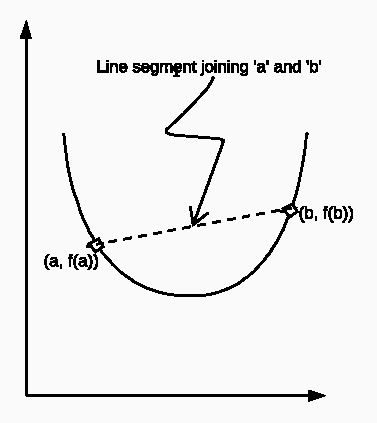
\includegraphics[scale=0.8]{fig1}
	\end{center}
	\end{frame}
	
	\begin{frame}{Example: $y = x^2$}
	Convex on the entire real line i.e. $(-\infty, \infty)$
	\begin{center}
	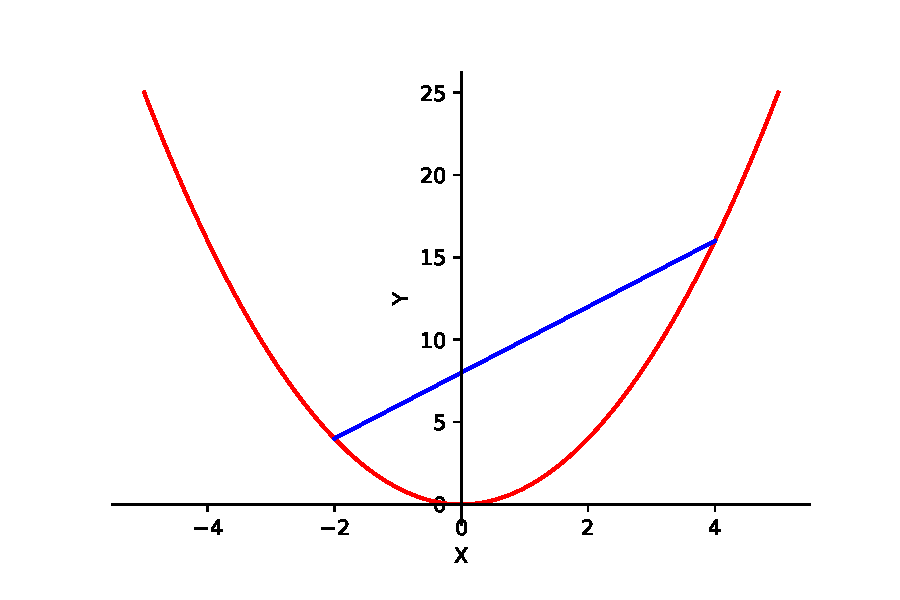
\includegraphics[scale=0.5]{y-x2}
	\end{center}
	\end{frame}

	\begin{frame}{Example: $y = |x|$}
	Convex on the entire real line i.e. $(-\infty, \infty)$
	\begin{center}
	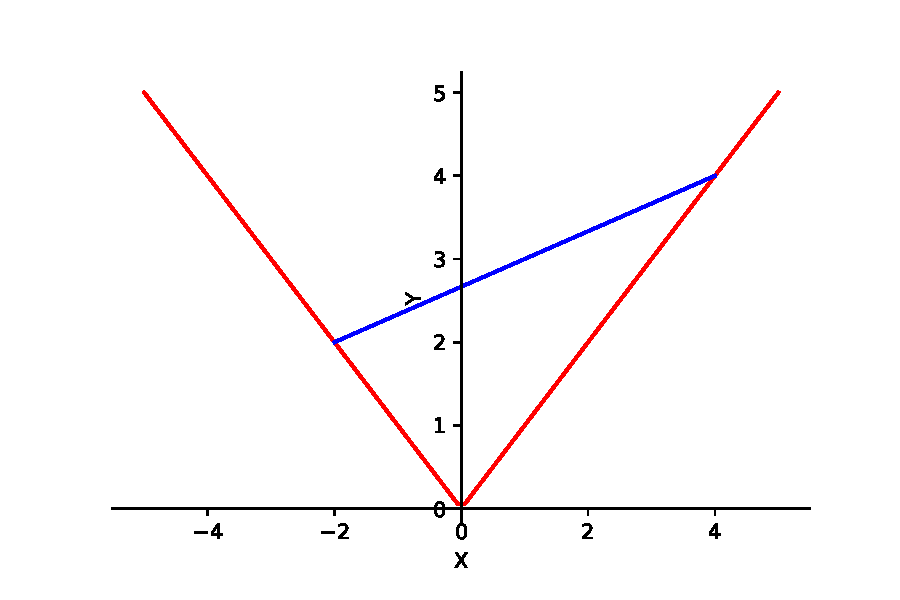
\includegraphics[scale=0.5]{y-absx}
	\end{center}
	\end{frame}

	\begin{frame}{Example: $y = e^x$}
	Convex on the entire real line i.e. $(-\infty, \infty)$
	\begin{center}
	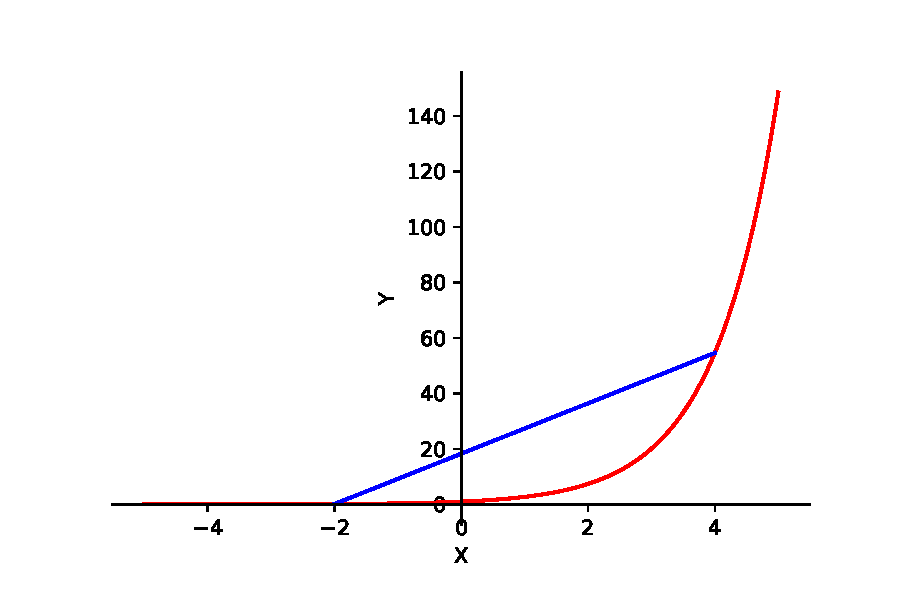
\includegraphics[scale=0.5]{y-ex}
	\end{center}
	\end{frame}

	\begin{frame}{Example: $y = \ln x$}
	Not convex on the entire real line i.e. $(-\infty, \infty)$
	\begin{center}
	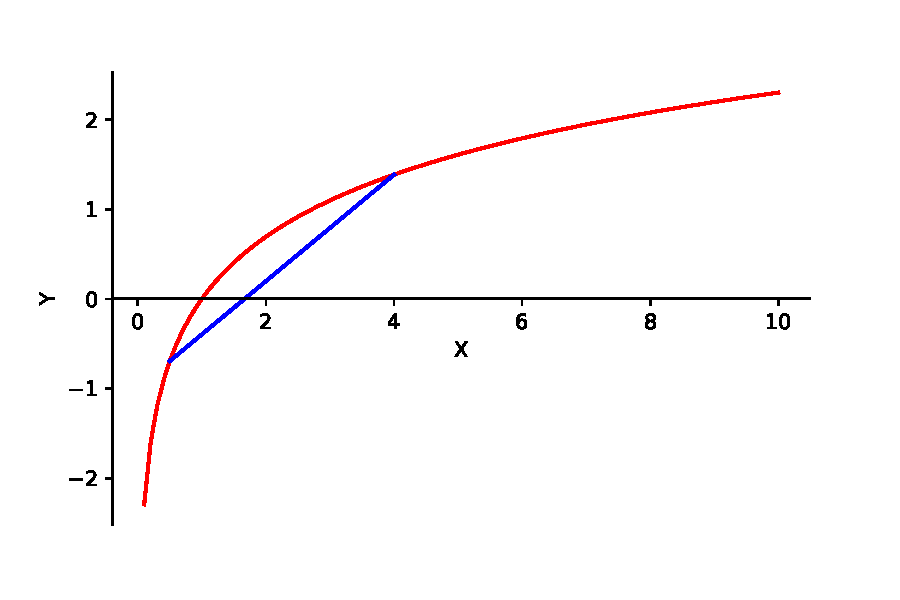
\includegraphics[scale=0.5]{y-logx}
	\end{center}
	\end{frame}

	\begin{frame}{Example: $y = x^3$}
	It is convex for the interval $[0,\infty)$
	\begin{center}
	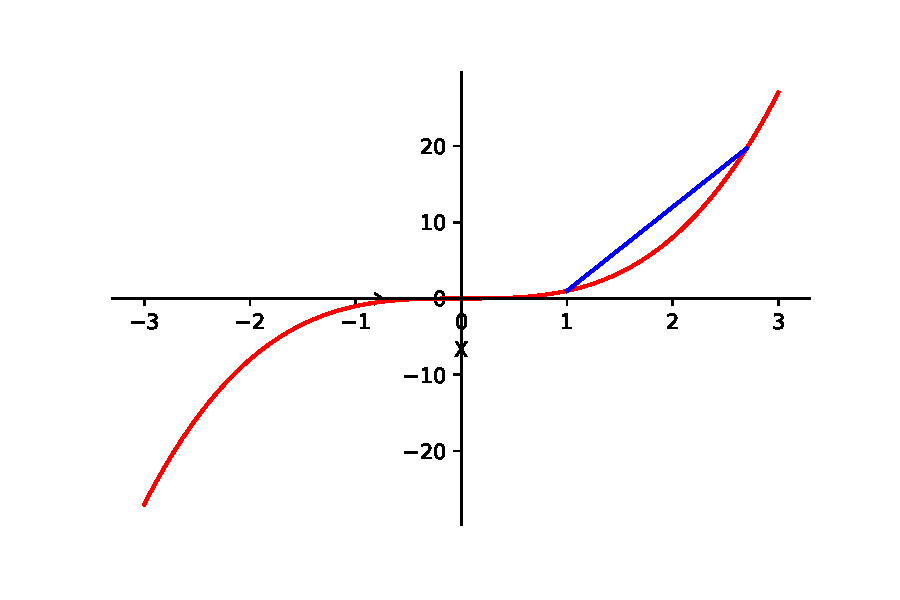
\includegraphics[scale=0.5]{y-x3_pos}
	\end{center}
	\end{frame}

	\begin{frame}{Example: $y = x^3$}
	It is concave for the interval $(-\infty, 0]$
	\begin{center}
	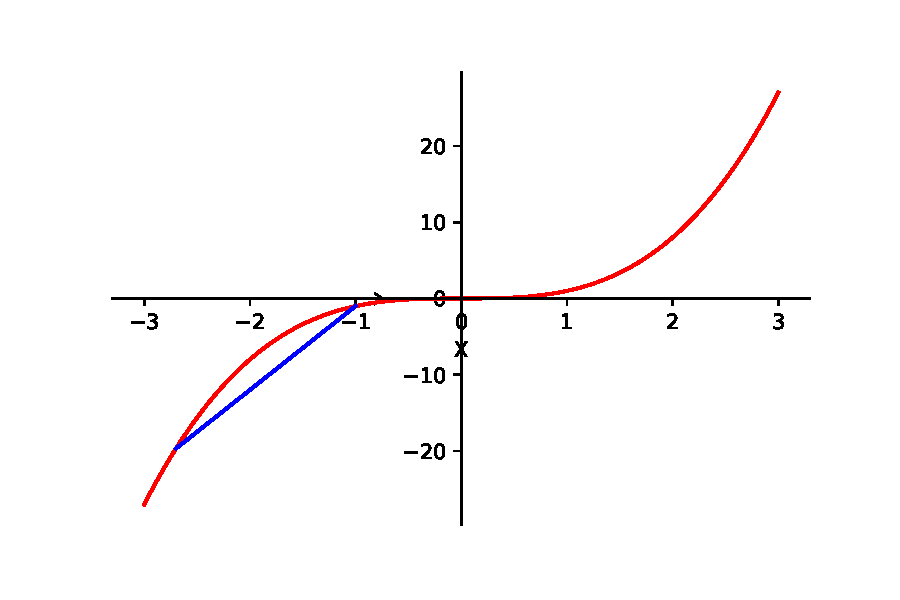
\includegraphics[scale=0.5]{y-x3_neg}
	\end{center}
	\end{frame}

	\begin{frame}{Example: $y = x^3$}
	But, it is not convex for the interval $(-\infty, \infty)$
	\begin{center}
	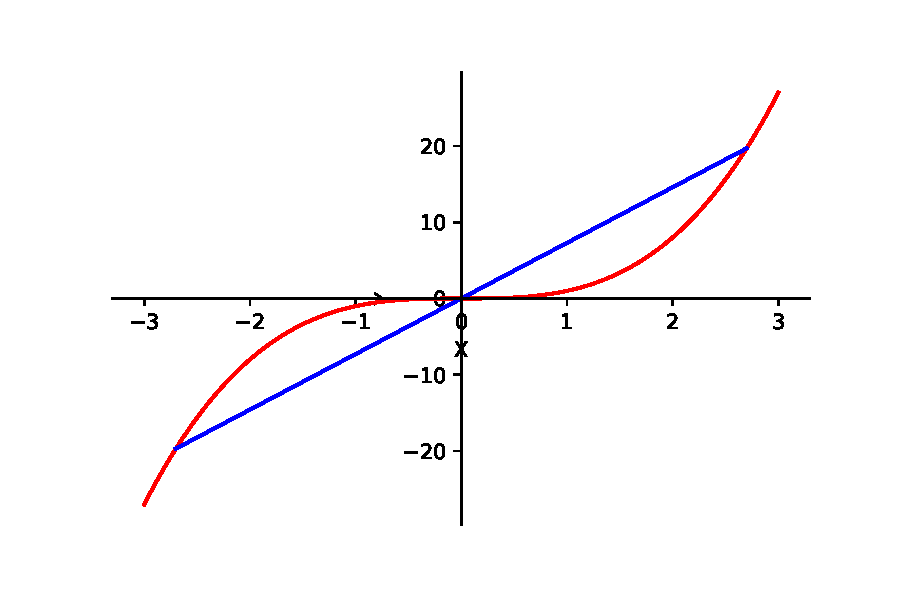
\includegraphics[scale=0.5]{y-x3}
	\end{center}
	\end{frame}

	\begin{frame}{Mathematical Formulation}
	Function $f$ is convex on set $X$, if $\forall x_1,x_2 \in X$ and $\forall t \in [0,1]$
	\begin{center}
	$f(tx_1 + (1-t)x_2) \leq tf(x_1) + (1-t)f(x_2)$\\
	\vspace{0.4cm}
	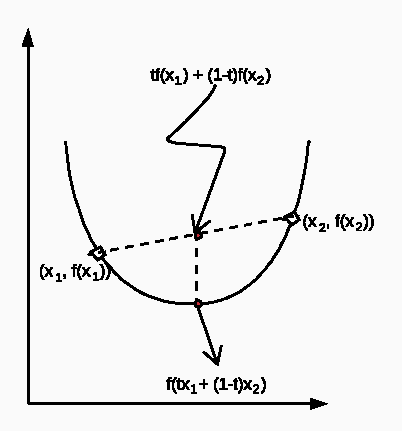
\includegraphics[scale=0.75]{proof_notation_fig}
	\end{center}
	\end{frame}


	\begin{frame}{Question: Prove that $f(x) = x^2$ is convex}
	\end{frame}

	\begin{frame}{Question: Prove that $f(x) = x^2$ is convex}
	\only<1-4>{To prove:
	\begin{center}
	$f(tx_1 + (1-t)x_2) \leq tf(x_1) + (1-t)f(x_2)$
	\end{center}
	}
	\only<2-4>{LHS = $f(tx_1 + (1-t)x_2)$ \hspace{0.5cm}=  $t^2x_1^2 + (1-t)^2x_2^2 + 2t(1-t)x_1x_2$\\
	RHS = $ tf(x_1) + (1-t)f(x_2)$ =  $tx_1^2 + (1-t)x_2^2$\\}
	\vspace{0.3cm}
	\only<3-4>{Here,\\
	LHS - RHS = $(t^2 -t)x_1^2 + [(1-t)^2 - (1-t)]x_2^2 + 2t(1-t)x_1x_2$ \\
	\hspace{1.8cm}               = $(t^2 - t)x_1^2 + (t^2 - t)x_2^2 - 2(t^2 - t)x_1x_2$\\
	\hspace{1.8cm}		      = $(t^2 - t)(x_1 - x_2)^2$ \\
	\vspace{0.3cm}
	}
	\only<4>{Here, $(t^2 - t) \leq 0$ since $t \in [0,1]$ and $(x_1 - x_2)^2 \geq 0$\\
	Hence, LHS -RHS $\leq$ 0\\
	Hence LHS $\leq$ RHS\\
	Hence proved.
	}
	\end{frame}


	\begin{frame}{Alternative ways to prove convexity}
	The Double-Derivative Test\\
	\vspace{1cm}
	If f''(x) $>$ 0, the function is  convex.\\
	\vspace{1cm}
	For example,\\
	\vspace{1cm}
	$\frac{\partial^2(x^2)}{\partial x^2} = 2 > 0 \Rightarrow x^2$ is a convex function.\\  
	\end{frame}

	\begin{frame}{Alternative ways to prove convexity}
	The double derivative test for multi-parameter function is equal to using the Hessian Matrix\\
	\vspace{1cm}
	A function $f(x_1,x_2,\ldots,x_n)$ is convex iff its $n \times n$ Hessian Matrix is positive semidefinite for all possible values of $(x_1,x_2,\ldots, x_n)$\\
	\begin{equation*}
\mH=\left[\begin{array}{cccc}
{\frac{\partial^{2} f}{\partial x_{1}^{2}}} & {\frac{\partial^{2} f}{\partial x_{1} \partial x_{2}}} & {\cdots} & {\frac{\partial^{2} f}{\partial x_{1} \partial x_{n}}} \\
{\frac{\partial^{2} f}{\partial x_{2} \partial x_{1}}} & {\frac{\partial^{2} f}{\partial x_{2}^{2}}} & {\cdots} & {\frac{\partial^{2} f}{\partial x_{2} \partial x_{n}}} \\
{\vdots} & {\vdots} & {\ddots} & {\vdots} \\
{\frac{\partial^{2} f}{\partial x_{n} \partial x_{1}}} & {\frac{\partial^{2} f}{\partial x_{n} \partial x_{2}}} & {\cdots} & {\frac{\partial^{2} f}{\partial x_{n}^{2}}}
\end{array}\right]
\end{equation*}
	\end{frame}


	\begin{frame}{Alternative ways to prove convexity}
	Show that $f(x_1,x_2) = x_1^2 + x_2^2$ is convex.\\
	\vspace{1cm} 
	\only<2->{
	\begin{equation*}
	\mH = 
	\begin{bmatrix}
		\frac{\partial^2(x_1^2 + x_2^2)}{\partial x_1^2} & \frac{\partial^2(x_1^2 + x_2^2)}{\partial x_1\partial x_2} \\
		 \frac{\partial^2(x_1^2 + x_2^2)}{\partial x_2\partial x_1} & \frac{\partial^2(x_1^2 + x_2^2)}{\partial x_2^2} \\
	\end{bmatrix}
	= 
	\begin{bmatrix}
		2 & 0 \\
		0 & 2\\
	\end{bmatrix}
	\end{equation*}\\
	}
	\only<3->{
	\vspace{1cm}
	Eigenvalues of $\mH$ are 2 and 2 $> 0 \Rightarrow$ $\mH$ is positive semidefinite.\\
	Hence, $f(x_1,x_2) = x_1^2 + x_2^2$ is convex. 
	}
	\end{frame}

	\begin{frame}{Convexity of linear least squares}
	Prove the convexity of linear least squares i.e. $f(\vtheta) = ||\vy - \mX\vtheta||^2$\\
	\vspace{0.5cm}
	\only<2->{
	We will use the double derivative (Hessian)\\
	\vspace{0.5cm}
	}
	\only<3->{
	$\frac{df}{d\vtheta} = \frac{d(||\vy||^2  - 2\vy^T\mX\vtheta + ||\mX\vtheta||^2)}{d\vtheta} = -2\vy^T\mX + 2(\mX\vtheta)^T\mX$\\
	\vspace{0.5cm}
	}
	\only<4->{
	$\frac{d^2f}{d\vtheta^2} = \mH = 2\mX^T\mX$\\
	\vspace{1cm}
	}
	\only<5->{
	$\mX^T\mX$ is positive semidefinite for any $\mX \in \Real^{m\times n}$.\\
	Hence, linear least squares function is convex.
	}
	\end{frame}


	\begin{frame}{Properties of Convex Functions}
	\begin{itemize}
	\item<1-> If $f(x)$ is convex, then $kf(x)$ is also convex, for some constant $k$
	\item<2-> If $f(x)$ and $g(x)$ are convex, then $f(x) + g(x)$ is also convex.
	\end{itemize}
	
	\only<3>{
	Using this we can say that:
	\begin{itemize}
	\item $(\vy-\mX\vtheta)^T(\vy-\mX\vtheta) + \vtheta^T\vtheta$ is convex 
	\item $(\vy-\mX\vtheta)^T(\vy-\mX\vtheta) + ||\vtheta||_1$ is convex 
	\end{itemize}
	}
	\end{frame}

\end{document}
